\chapter{研究背景}
\label{章:研究背景}
臺灣是多元民族的國家,
逐家攏有家己的文化,
逐个民族講的話攏無仝,
有人講閩南語,
有人講泰雅語,
有人講客話,……,
最近二十幾年來閣有越南話、印尼話、……
新住民\footnote{佇2013年提著中華民國國籍5004人中,對越南來的3855人,對印尼來的566人\cite{國籍之歸化取得人數}}的語言。
臺灣語言主要會當分做南島語(Austronesian)佮漢語(Chinese)兩種\footnote{新住民的越南語是南亞語系,泰國話是狀侗語系}。

南島語是全世界分布上闊的語族\cite{臺灣原住民史李壬癸},
上北爿到臺灣、南爿到紐西蘭,東爿到復活節島,西爿到馬達加斯加。
民族語言網\cite{Ethnologue}共南島語會當分做十个族群,
臺灣摻蘭嶼這十个族群攏有,
語系變化誠大,
代表臺灣佇南島語的研究內底非常重要,
所以臺灣的原住民語系變化誠大。


\includegraphics[height=1em]{字/⿰因}閣比漢人較早到臺灣,才會予人叫原住民。
佇歷史的文書記錄面頂,十七世紀荷蘭佮西班牙來臺灣進前就有一个幾仔族原住族組合起來的大肚王國\cite{中研院民族所數位典藏大肚番王傳奇},
\ji{⿰因}保護\ji{⿰因}家己的土地,
抵抗荷蘭人,鄭成功政權,清國的統治,
到大甲西社事件才滅國。
到今仔日,
臺灣的原住民除了中華民國政府的原民會認定的十六族以外,
閣有誠濟猶未認定的族,
親像臺南的西拉雅佮埔里的噶哈巫……,
攏總有二三十族以上。

臺灣用的漢語主要會當分做三大種,
閩南語、客家話佮官話\cite{外省族群的母語與國語}。
閩南語佮客家話是對四百外年前開始,
佇明國、清國的福建人因為枵腹肚蹛袂落,
姑不而將駛船渡過烏水溝\footnote{又叫臺灣海峽},
來臺灣趁食。
佇清國的時陣透過政治佮經濟的力量一步一步食掉原住民的土地,
上尾佇臺灣變做上大的族群之一。

講著閩南語的文字,
定定有人問:「閩南語是欲按怎寫!?」
除了用拼音的方式寫出來以外,
閩南語有九成以上是有漢字的\cite{洪惟仁閩南語九成有漢字},
鶴佬人\footnote{閩南人。漢字有爭議,教育部無訂落來,採用洪惟仁教授的用字慣勢}祖先搬去閩越地區時,
就佮遐的壯苗族原住民通婚,
因為原住民人濟,
所以予鶴佬人同化的時留落來這一寡毋是漢語的詞,
董忠司\cite{董忠司非漢語初探}認為「查甫」佮「查某」的「查」,
「大家」佮「大官」的「大」是狀侗族的詞頭。
雖然「查」大部份人攏讀「tsa」,毋過佇臺灣漢語辭典\cite{臺灣漢語辭典}有記錄「ta」的音,佮「大」仝音
%加注音

張光宇\cite{閩客方言史稿}研究歷史音韻學佮聲韻學\footnote{相關理論請看\ref{節:音韻學}節佮\ref{節:漢語聲韻學}節}認為,
閩南語的漢語部份是西晉後尾動亂的兩擺大移民、
唐朝陳元光𤆬兵鎮壓狀苗族原住族,
佮南宋時期文教影響,
攏總四擺移民,佮政府制度影響,
造成四層漢語語言層的閩南語。
頭前三層語言層的語音叫做白話音,
上尾第四擺後南宋音號做文讀音,
親像「石」這个字,
有「\tsoo{石}{⿳⿳⿳⿳ㄐㄧㄜ㆐ㆷ}{tsioh8}\tsoo{頭}{⿳⿳ㄊㄠˊ}{thau5}」、
「\tsoo{石}{⿳⿳⿳⿳ㄒㄧㄚ㆐ㆷ}{siah8}\tsoo{榴}{⿳⿳⿳ㄌㄧㄨˊ}{liu5}」\footnote{一種果子}、
「\tsoo{藥}{⿳⿳⿳ㄧㆦ㆐ㆶ}{iok8}\tsoo{石}{⿳⿳⿳ㄒㄧ㆐ㆶ}{sik8}」\footnote{方藥與砭石兩種藥仔}三種語音,
佇語言是規律變化的假設之下,
這个「石」字就代表上少有三層語言層。

客家話這馬佇臺灣較大腔口有「四海大平安」\footnote{四縣腔、海陸腔、大埔腔、饒平腔、詔安腔}。
鶴佬人佮客人毋管佇亞洲大陸抑是臺灣,
生活攏無遠,誠濟詞的用法攏相像,
親像閩南語講「\tsoo{頭}{⿳⿳ㄊㄠˊ}{thâu}\tsoo{前}{⿳⿳⿳ㄐㄧㄥˊ}{tsîng}」,
四縣客話講「\tsoo{頭}{}{teuˇ}\tsoo{前}{}{qienˇ}」\footnote{客話拼音會當看客話拼音\cite{客話拼音},意思會當查客話辭典\cite{客話辭典}},
閩南語講「\tsoo{好}{⿳⿳ㄏㄜˋ}{hó}\tsoo{勢}{⿳⿳ㄙㆤ˪}{sè}」,
四縣客話嘛講「\tsoo{好}{}{hoˋ}\tsoo{勢}{}{se}」。

佇臺灣的鶴佬人佮客人來臺灣佮原住民通婚,
生活中嘛濫著原住民的用詞,
親像「臺灣」是西拉雅語「Taian」或「Tayan」對外地人的稱呼\cite{台灣名稱的由來},
咱定定食著的「菝仔」嘛是平埔族話\cite{客語外來語}。

%%%%
毋但原住民話,
閩南語佮客話嘛有佮別的語言交插,
像是的「六甲地」的「甲」是從荷蘭「akker」來的\cite{台甲}。
受過日本的統治,
閩南語佮客話攏有濫著日語,
親像「臭柿仔」,日語唸「\tsoo{トマト}{}{tomato}」,
閩南語閣會當講「kha7*-ma1*-tooh*」\footnote{音標有*代表外來詞,頭前兩音節kha7、ma1免閣變調},
客話講「」,「オ-トバイootobai」閩南語講「機車」「oo1-too」,
客話講。
會當講是臺灣的歷史攏藏佇臺灣的語言內底。

%%%%%%%%%

上尾一个漢語官話是中華民國政府拍輸中國人民共和國了,
𤆬誠濟中國人來臺灣,
因為逐个的故鄉攏無仝\cite{外省族群的母語與國語},
民國政府就繼續用佇亞洲大陸的規範,
共北京官話的語音、白話文的用法當做基礎,
利用政府機關,教育認知\footnote{本人阿姨有佇學校講母語予人罰過錢}、…等手法佇臺灣捒,
所以華語這馬是佇臺灣是有上政治優勢的語言。
毋過這馬佇臺灣實際用的官話閣佮北京用的官話無仝款,
有加入臺灣本土的元素,是北京官話的次方言之一。
除了這三種漢語以外,
佇二次大戰了中華民國政府𤆬來臺灣的人,
\ji{⿰因}的母語嘛誠濟種\cite{外省族群的母語與國語},
毋過這馬攏已經消失甲差不多矣。

為著方便起見,本論文下跤的閩南語佮客話攏是講佇臺灣用的閩南語佮客話,
官話就照中國海外華人的慣勢,稱呼佇臺灣使用的北京官話次方言做華語。
%中華民國政府就暫時叫做用政府,中華民國政府的教育部號做教育部。
本論文主要用閩南語寫,毋過會用著一寡華語佮客話。
為著格式一致,予人有法度一看就知影是啥物語言,
閩南語會用「臺羅拼音\cite{臺羅拼音}佮方言音符號\cite{華、台語注音符號溯源}」,
客話會用「客話拼音\cite{客話拼音}」,
華語會用「注音符號\cite{華、台語注音符號溯源}」。
引用的閩南語的羅馬拼音攏會轉臺羅,
毋過人名、文章名、冊名保持原樣。

\section{研究目的}
\label{節:研究目的}
%母語重要→資料無夠→需要翻譯→整理翻譯語料
最近十幾冬政府開始注重人權,講母語是人上基本的權利,
毋但國校仔國中攏開始有鄉土語言的課矣\footnote{除了本土語言以外,閣有新住民語言},
逐家嘛開始研究母語\footnote{請看\ref{章:相關研究}章},
毋過定定會拄著文字、語料、教材數量無夠的問題。

親像電視台想欲製做母語的新聞,毋過大部份攏是華語的材料;
學生想欲知影華語一句話,母語按怎講,
%文字空課
%翻譯本身
%隨身翻譯機
%數位資料無夠→翻譯重要
%外地人到臺灣,聽無臺灣話,
這時陣就會當利用華語資料攏誠濟的優勢,
共華語翻譯做母語,按呢就會解決這幾項問題。

這馬翻譯的技術已經發展到一个坎站矣,
毋過華語翻譯做母語的效果攏無蓋好,
主要是母語的語料數量無夠,
本論文就針對華語到閩南語的翻譯,
研究按怎處理數量有限的閩南語語料,予翻譯閣較好。
予後壁的人會使利用這个成果,繼續研究閩南語,
抑是會當利用這篇文章的經驗,推廣到別的臺灣語言,
上直接的,就是會當予母語使用者有閣較方便的數位環境。

%%看按怎順
%若是閣配合語音模型\footnote{請看\ref{章:語音模型}},
%都會使做一个即時口語翻譯系統。
%第一線佇學校教冊的老師需要電子化的翻譯,
%抑是關心母語的文字工作者,
%攏會使利用這个研究成果繼續做落去。

\section{語料狀況}
\label{節:語料狀況}
佇處理閩南語語料進前,都愛先了解閩南語語料的歷史。

上早的閩南語文體是明國時代流傳落來的荔鏡記戲文\cite{荔鏡記戲文研究──校勘篇},
清國時代有閣較濟的字典、歌仔冊佮教會詩歌,
日本時代開始有人感受閩南語消失的威脅,產生出臺灣話文論戰,
到中日戰爭開始,日本人禁止用漢文。%愛閣順過
中華民國政府來臺灣隨就二二八,臺灣文學因為白色恐佈,
到最近二十幾冬,閩南語就開始有大量的文章

因為歷史誠久長,
閩南語的書寫方式有誠濟種,會當分做三種。
第一種全部用漢字,叫做全漢,
就全部用漢字表達閩南語,
因為閩南語有部份毋是漢語,
拄著這種情形逐家用的漢字攏無仝,
到最近幾冬,才有教育部以官方單位規範用字\footnote{臺灣閩南語推薦用字700字表\cite{臺灣閩南語推薦用字700字表},佇96~99年公佈修正}。

第二種是用拼音,
佇清國時期,來傳教的傳教士為著學閩南語,佮鶴佬人講話,
定一套閩南語的羅馬拼音,一般號做「教會羅馬拼音」\footnote{幾仔个版本,一般是講X的版本}
日本時期,日本政府嘛是為著統治原因,
用日本的aiueo來記錄\footnote{台日、日台大辭典}。
到中華民國時期,
有模仿華語注音符號的方言音符號,
最近幾十年,有主張佮英文系統較倚的通用拼音,
上尾教育部改教羅羅馬拼音的缺點\footnote{毋是一擺就改好,中央閣有TLPA拼音},
號做「臺灣羅馬字拼音」,後壁號做「臺羅」。
因為這馬羅馬拼音較有優勢,所以本論文共全部用拼音的文章攏叫做「全羅」。

面頂兩種攏有一个缺點,
就是上深的漢字抑是全篇的拼音對一般人來講較歹接受,
第三種是共漢字佮拼音濫做伙,
主要是漢字,拄著較歹寫抑是揣無本字的漢字,
就寫拼音。

\section{論文貢獻}
\label{節:論文貢獻}
%第一个問題是 我們提出XX演算法
%第一个問題是翻譯語料有限,會出現「未知詞問題」,本論文提出「拄好長度斷詞」的演算法,改良斷詞的效果。
%第二个問題是翻譯語料型式真濟款,提供的資料嘛無仝,本論文提出「互相整理」的演算法,予語料格式統一。%愛號名
%第三个問題是網路語料華語閩南語濫做伙,需要共分開,以早研究攏是針對拼音字母,本論文是針對漢語方言,加特徵詞,幫助分類。
本論文主要有四个對翻譯語料的貢獻,
第一个是本論文提出「拄好長度斷詞」的演算法。
第二个貢獻是比較漢語語料樣式對翻譯的影響,
比較斷詞佮斷字翻譯模型,
佇按怎的組合之下效果上好。
第三个是提出一个自動整理漢語語料的方法,
予資訊無完整的語料庫補足資訊,
發揮上大的價值。
上尾一个是提出分類兩種漢語的方法,
免用傷濟特徵詞就會當得著袂的翻譯效果,
佇網路頂掠落來的資料就有法度分類。

\section{論文架構}
\label{節:論文架構}

%\begin{figure}
%\centerline{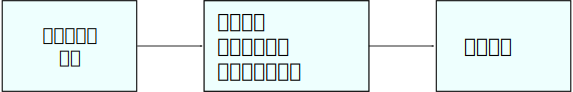
\includegraphics[keepaspectratio]{圖/規个論文}}
%\caption{本論文希望揣出自動整理語料的方法,予翻譯效果閣較好}
%\label{圖:規个論文架構}
%\end{figure}
%圖\ref{圖:規个論文架構}是這篇論文的架構,圖中央是本論文愛處理的三个問題,分別寫佇第三、四、五章。
第\ref{章:研究背景}章介紹臺灣語言的現況佮特徵,研究的動機佮論文研究的方向佮重點。
第\ref{章:相關研究}章介紹語言相關學術研究佮技術原理。
第\ref{章:研究介紹}章定義本篇論文愛處理的問題,
第\ref{章:研究方法}章提出一寡方法,解決頂一章翻譯語料的問題。
第\ref{章:實驗結果}章做實驗而且驗證結果。
第\ref{章:實驗結果}章寫按怎分別網路頂的臺語佮華語資料。
上尾的結論佮以後會當發展的方向攏記佇第\ref{章:結論佮未來發展}章。
